\begin{slide}

\large{Go\'{e}LUG} \hfill \small{Linux User Group - Le Havre} \\
Conférence le \texttt{04-Fevrier-2016} \hfill \texttt{http://www.goelug.org} %
%
%
\begin{tikzpicture}[remember picture, overlay]
\node at (current page.north west){%
\begin{tikzpicture}[overlay]
\node[opacity=0.2, anchor=west] at (50mm,-50mm) {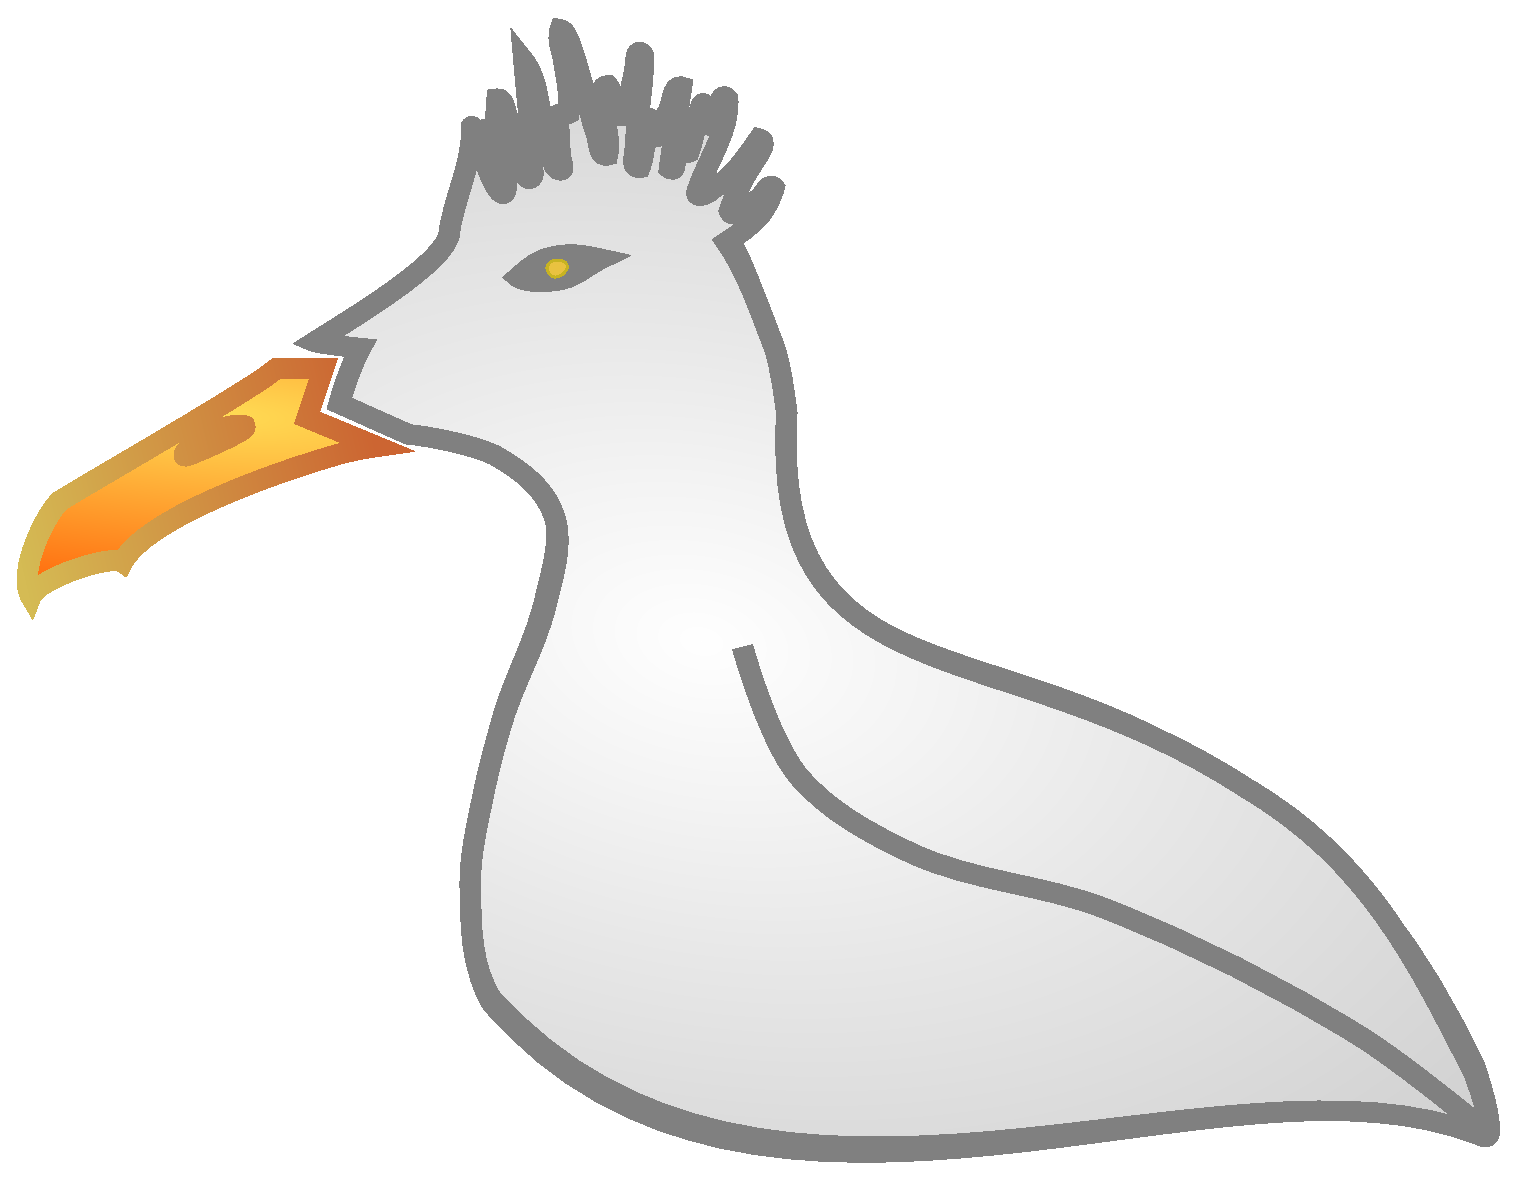
\includegraphics[scale=0.35]{../goeland}};
\end{tikzpicture}
};
\end{tikzpicture}
%
\begin{center}
    \large{Un F.A.I. associatif au Havre ?} \\
    \large{Go\'{e}LUG vous invite pour la présentation de la} \\
    \huge{Fédération FDN} \\
    \textbf{\em{\large{F}\normalsize ournisseurs d'\large{A}\normalsize cc\`es \large{I}\normalsize{nternet} associatifs}}
\end{center}
%
{\small
Internet et le Logiciel Libre sont indissociables : sans l’un, l’autre ne peut plus vraiment marcher. C’est pourquoi il est important que, nous autres libristes, nous prenions un peu notre Internet en main. La FFDN regroupe actuellement vingt-sept fournisseurs d’accès associatifs, qui amènent du vrai Internet neutre et transparent un peu partout en France et en Belgique\dots mais il s’agit d’associations locales, et il en manque encore une qui soit basée en Normandie. \\
Dans cette conférence, nous parlerons des enjeux rendant nécessaire de monter un tel FAI normand, et regarderons de plus près quelques exemples de ce que font les membres de la fédération, et qui pourraient être mis en place au Havre et aux alentours.
}
%
\begin{center}
Le \texttt{04-Fevrier-2016} \texttt{20h00} \\
A la cantine numérique \texttt{LE CONTAINER}
\end{center}
%
\begin{center}
\texttt{
https://www.ffdn.org/fr \\
http://www.lecontainer.co
}
\end{center}
%
\end{slide}